\documentclass{beamer}
\usepackage[T1]{fontenc}
\usepackage[utf8]{inputenc}
\usepackage{natbib}
\usepackage{bibentry}

\usepackage[francais]{babel}
\usepackage{graphicx}
\usepackage{geometry}
\usepackage{eurosym}


\usepackage{comment}

\graphicspath{{./Figures/}{./Animations/}}

\mode<presentation> {
	\usetheme{Singapore}
	%\usetheme{Madrid}
}



\def\onedot{$\mathsurround0pt\ldotp$}
\def\cddot{% two dots stacked vertically
	\mathbin{\vcenter{\baselineskip.67ex
			\hbox{\onedot}\hbox{\onedot}}%
}}



\newcommand{\matr}[1]{\bm{#1}} 

\newcommand{\blue}[1]{\textcolor{blue}{#1}}
\newcommand{\red}[1]{\textcolor{red}{#1}}
\newcommand{\green}[1]{\textcolor{red}{#1}}

% make bibliography entries smaller
%\renewcommand\bibfont{\scriptsize}
% If you have more than one page of references, you want to tell beamer
% to put the continuation section label from the second slide onwards
%\setbeamertemplate{frametitle continuation}[from second]
% Now get rid of all the colours
%\setbeamercolor*{bibliography entry title}{fg=black}
%\setbeamercolor*{bibliography entry author}{fg=black}
%\setbeamercolor*{bibliography entry location}{fg=black}
%\setbeamercolor*{bibliography entry note}{fg=black}
% and kill the abominable icon
%\setbeamertemplate{bibliography item}{}


\expandafter\def\expandafter\insertshorttitle\expandafter{%
	\insertshorttitle\hfill%
	\insertframenumber\,/\,\inserttotalframenumber}


\title[Collaboration avec l'ITA]{Presentation mobilité doctorale à l'ITA \\ (Istituto Tecn\'ologico de Aeron\'autica)}
\author[A. Brugnoli ISAE-SUPAERO]{\small Andrea Brugnoli \\
 \footnotesize Directeurs des Theses: Daniel Alazard (ISAE-SUPAERO), Valerie Pommer-Budinger (ISAE-SUPAERO) \\
\footnotesize Encadrant à l'ITA: Flavio Luiz Cardoso Riberio}
%\date{23 janvier 2014}

% Clear the navigation bar
\setbeamertemplate{navigation symbols}{}
%\setbeamercolor{section in head/foot}{fg=black, bg=white} 




%\AtBeginSection[]
%{
%	\begin{frame}<beamer>
%	\frametitle{Outline}
%	\tableofcontents[sectionstyle=show/shaded, subsectionstyle=show/show/hide]
%\end{frame}
%}

%\AtBeginSubsection[]
%{
%\begin{frame}<beamer>
%\frametitle{Outline}
%\tableofcontents[sectionstyle=show/shaded, subsectionstyle=show/shaded/hide]
%\end{frame}
%}



\begin{document}
	
	
\begin{frame}
	\titlepage
\begin{columns}
	\begin{column}{0.5\textwidth}
		\centering
		
\includegraphics[height=0.2\textheight]{ISAE-SUPAERO.png}
	\end{column}
	\begin{column}{0.5\textwidth}
		\centering
		
\includegraphics[scale=0.3]{ITA_logo.png}
	\end{column}
\end{columns}
\end{frame}


\section{Ma mobilité}
\begin{frame}{Mobilité, pourquoi faire?}
\begin{columns}
	\begin{column}{0.5\textwidth}
		Mes raisons
		\begin{itemize}		
		\item sortir de ma routine;
		\item me confronter avec une réalité très différente;
		\item pouvoir travailler avec une personne jeune qui connaît bien mon sujet;
		\end{itemize}
		Mes suggestions
		\begin{itemize}
			\item{C'est une occasion. Profitez-en.}
		\end{itemize}
	\end{column}
	\begin{column}{0.5\textwidth}
		\centering
		\includegraphics[scale=0.9]{trip_sjc.eps}
	\end{column}
\end{columns}
\end{frame}

\begin{frame}{Le Brésil}
\only<1>{
\begin{figure}
\centering
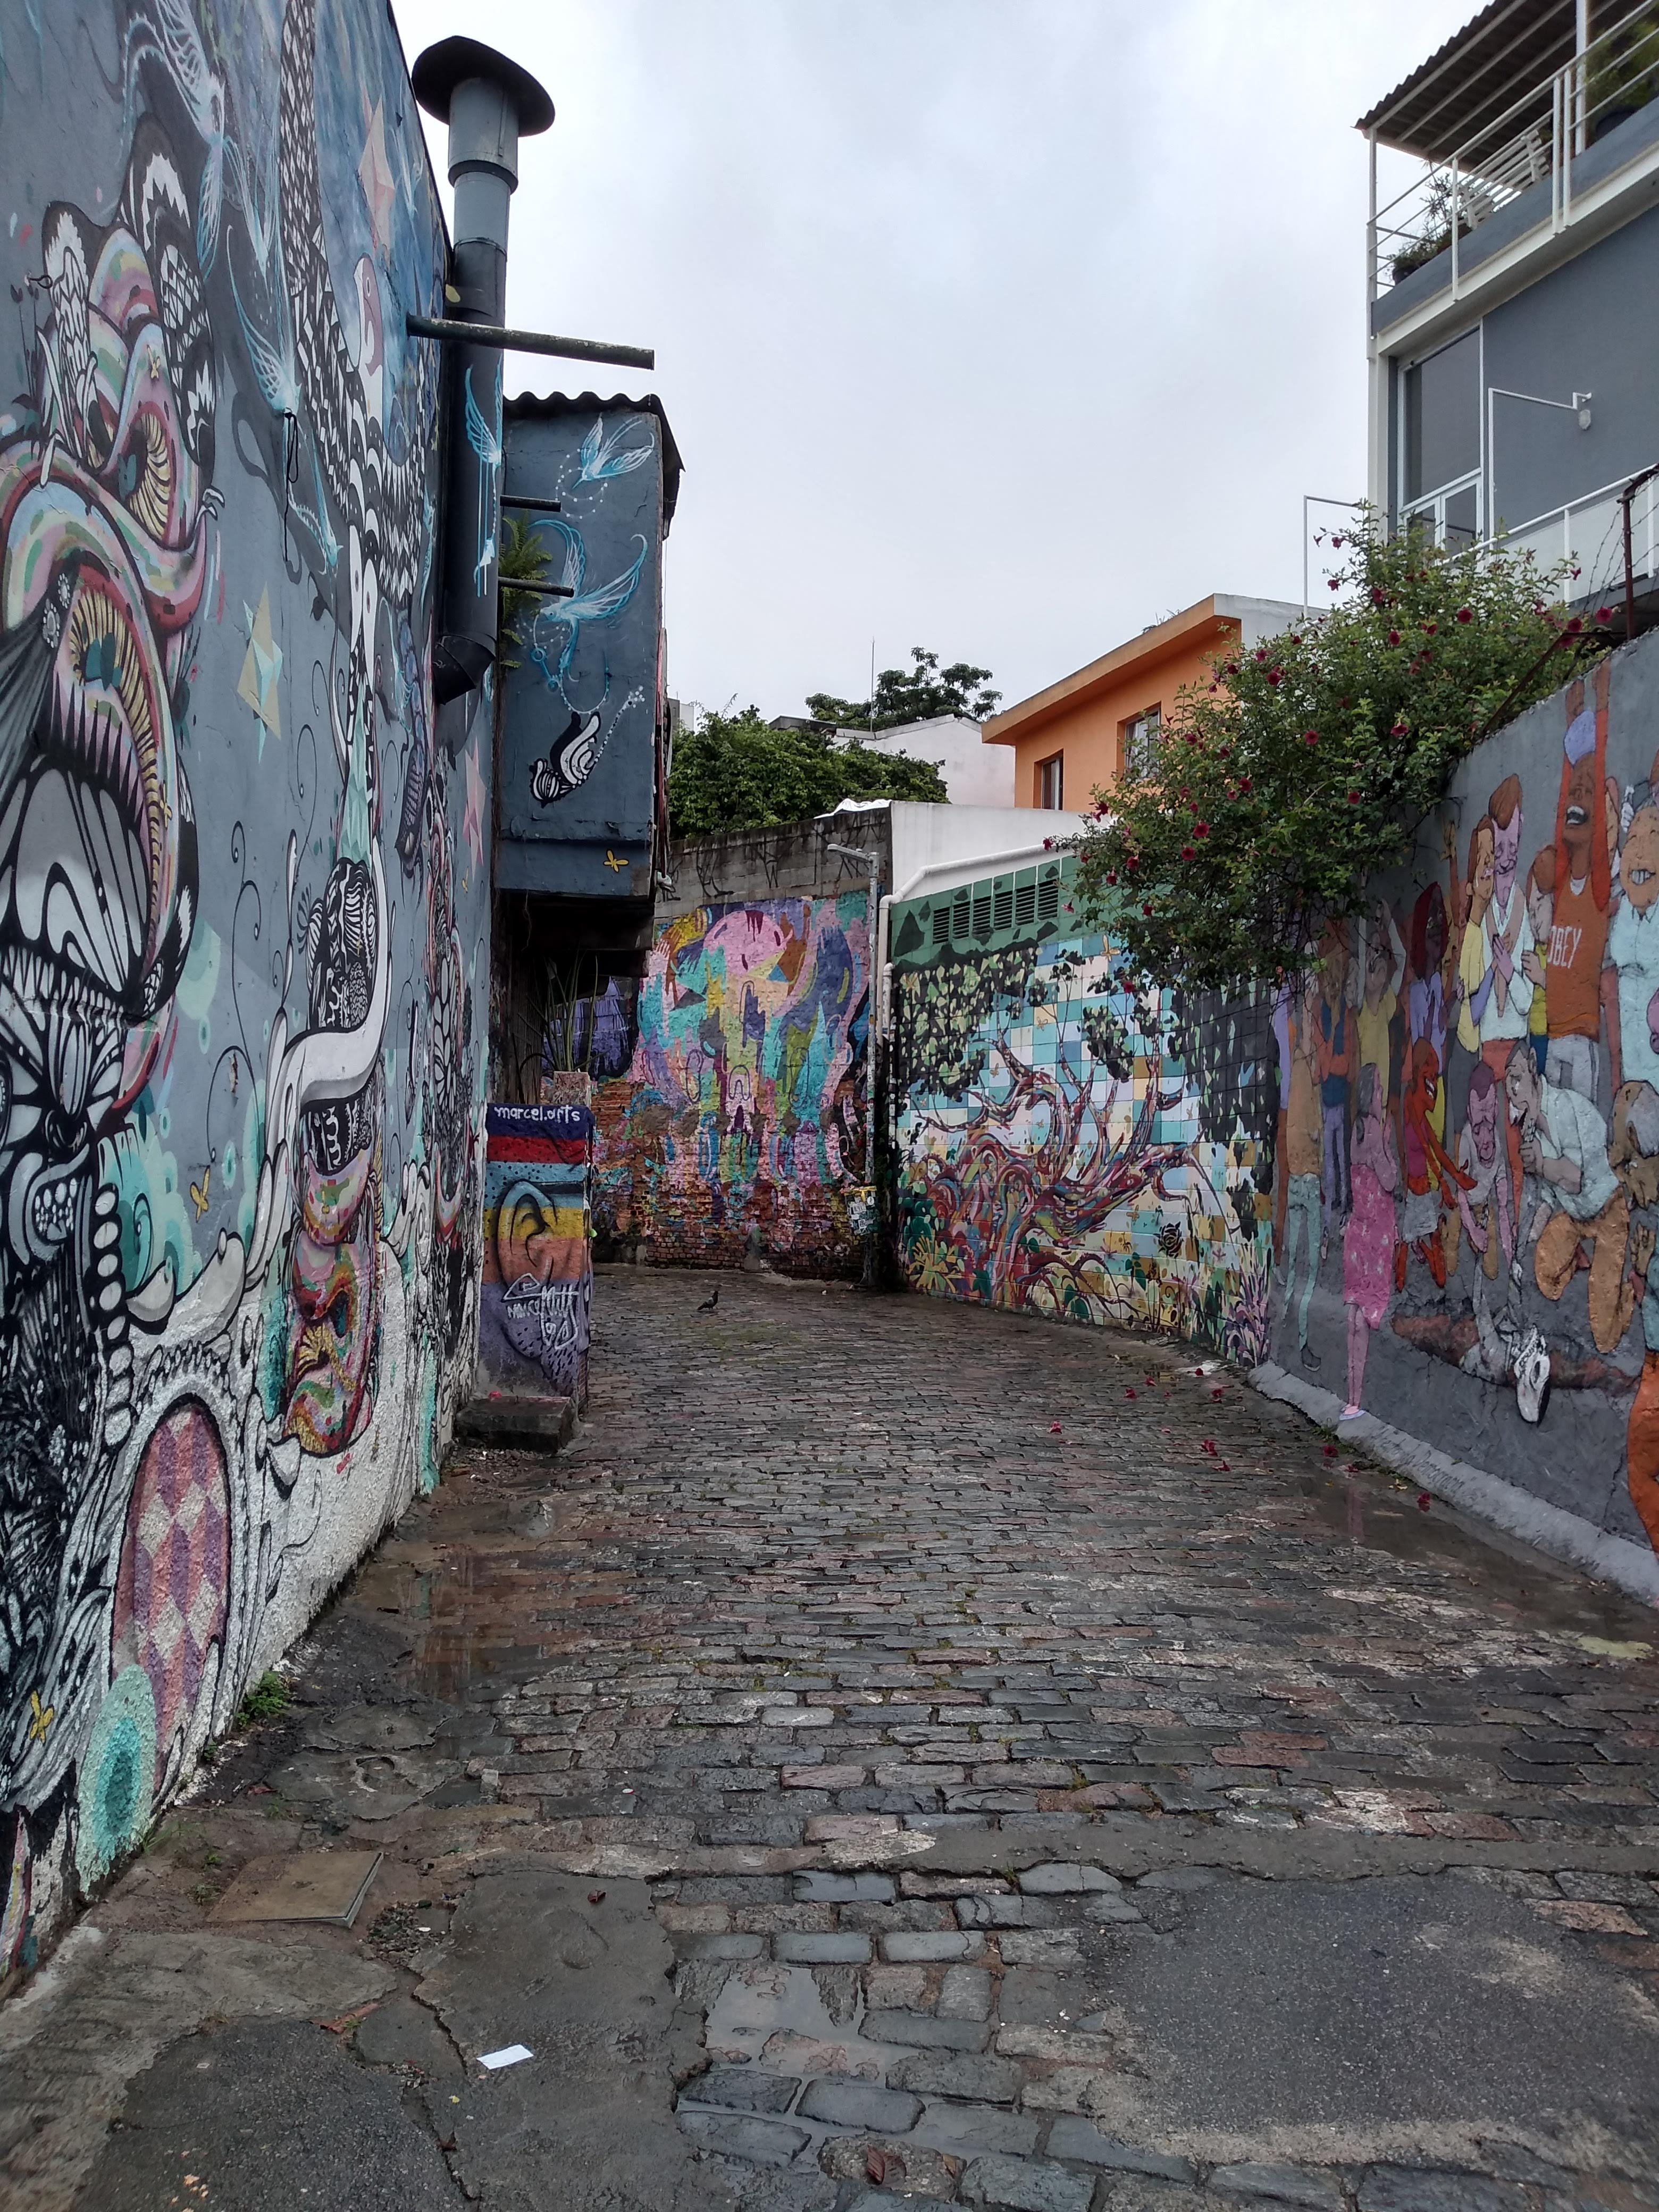
\includegraphics[height=.8\textheight]{beco_batman.jpg}\caption{Beco do batman, S\~ao Paulo}
\end{figure}
}	
\only<2>{
\begin{figure}
\centering
\includegraphics[height=.8\textheight]{Sao_paulo.jpg}\caption{Pinacoteca, S\~ao Paulo}
\end{figure}	
}
\only<3>{
	\begin{figure}
		\centering
		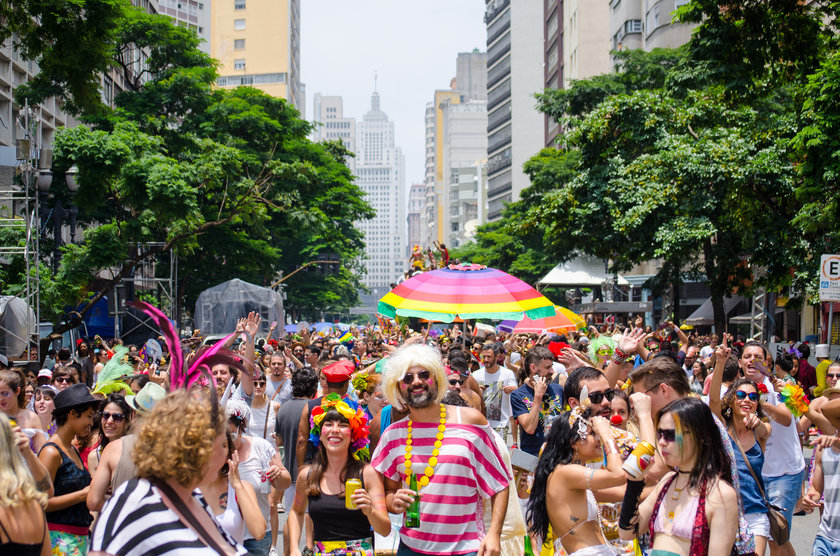
\includegraphics[height=.8\textheight]{carnaval-sao-paulo.jpg}\caption{Avenida Paulista, S\~ao Paulo}
	\end{figure}
}
\only<4>{
\begin{figure}
\centering
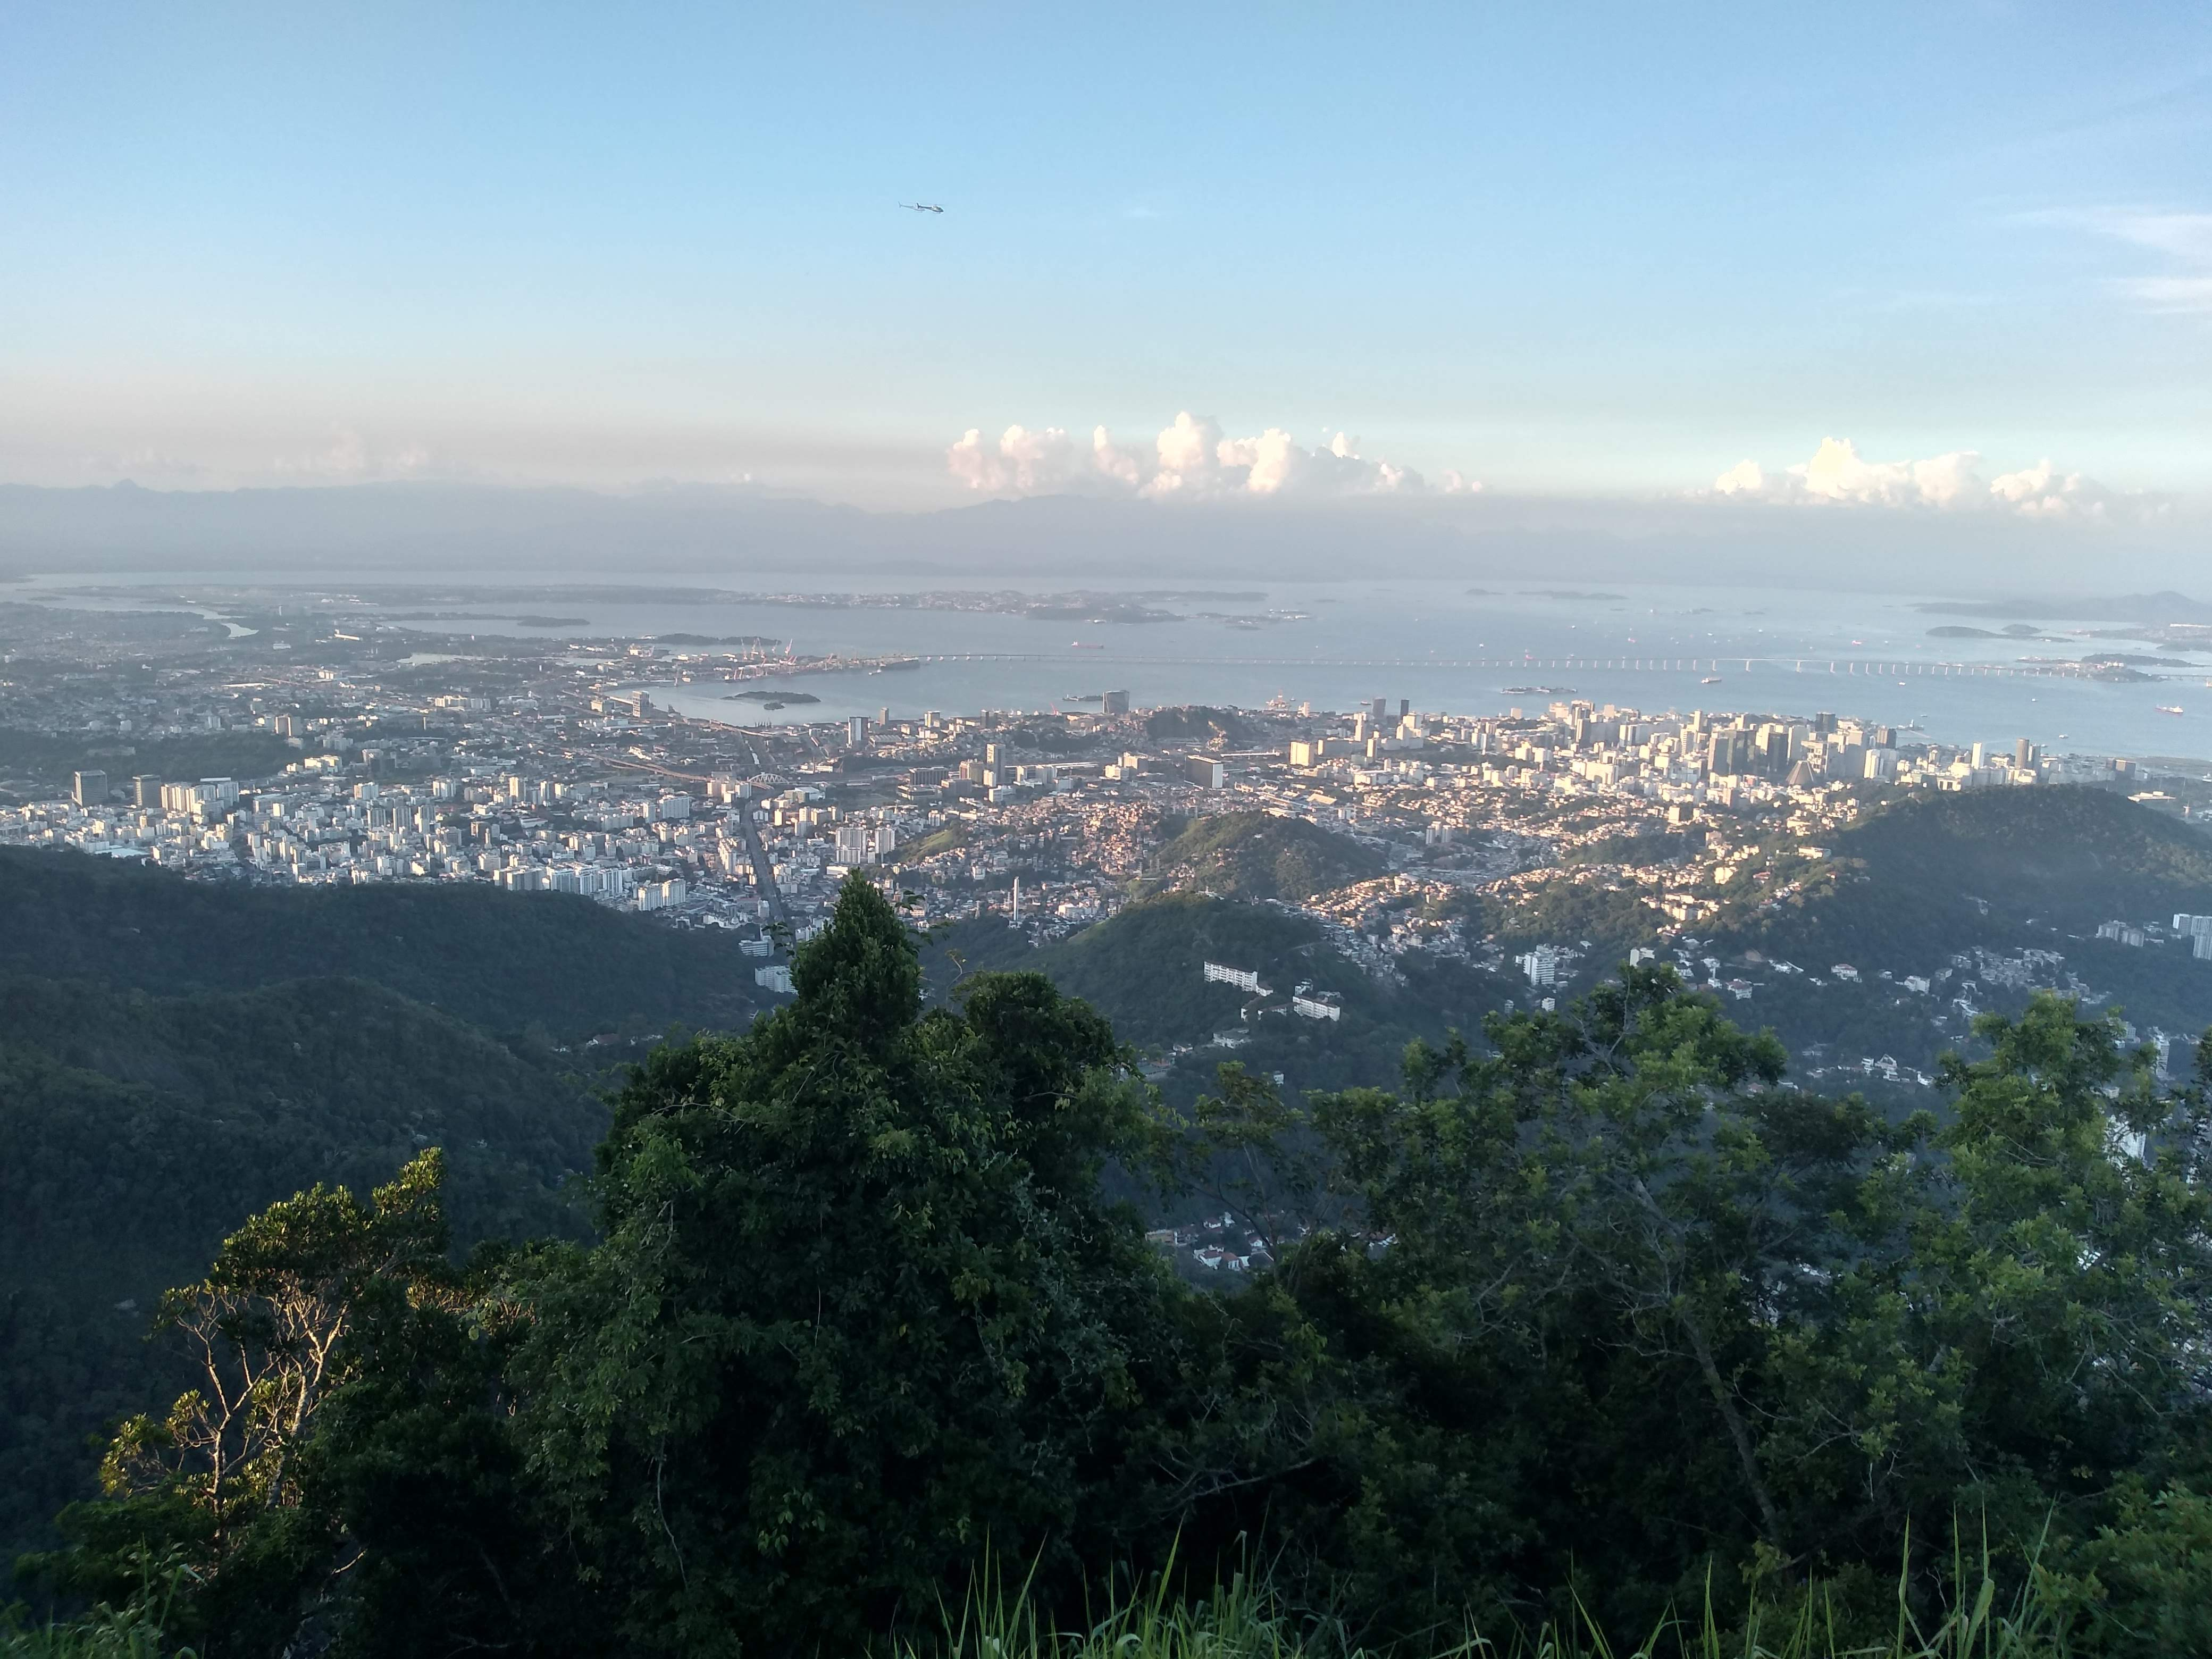
\includegraphics[height=.8\textheight]{Rio_cristo.jpg}\caption{Cristo Redentor, Rio de Janeiro}
\end{figure}
}
\only<5>{
\begin{figure}
\centering
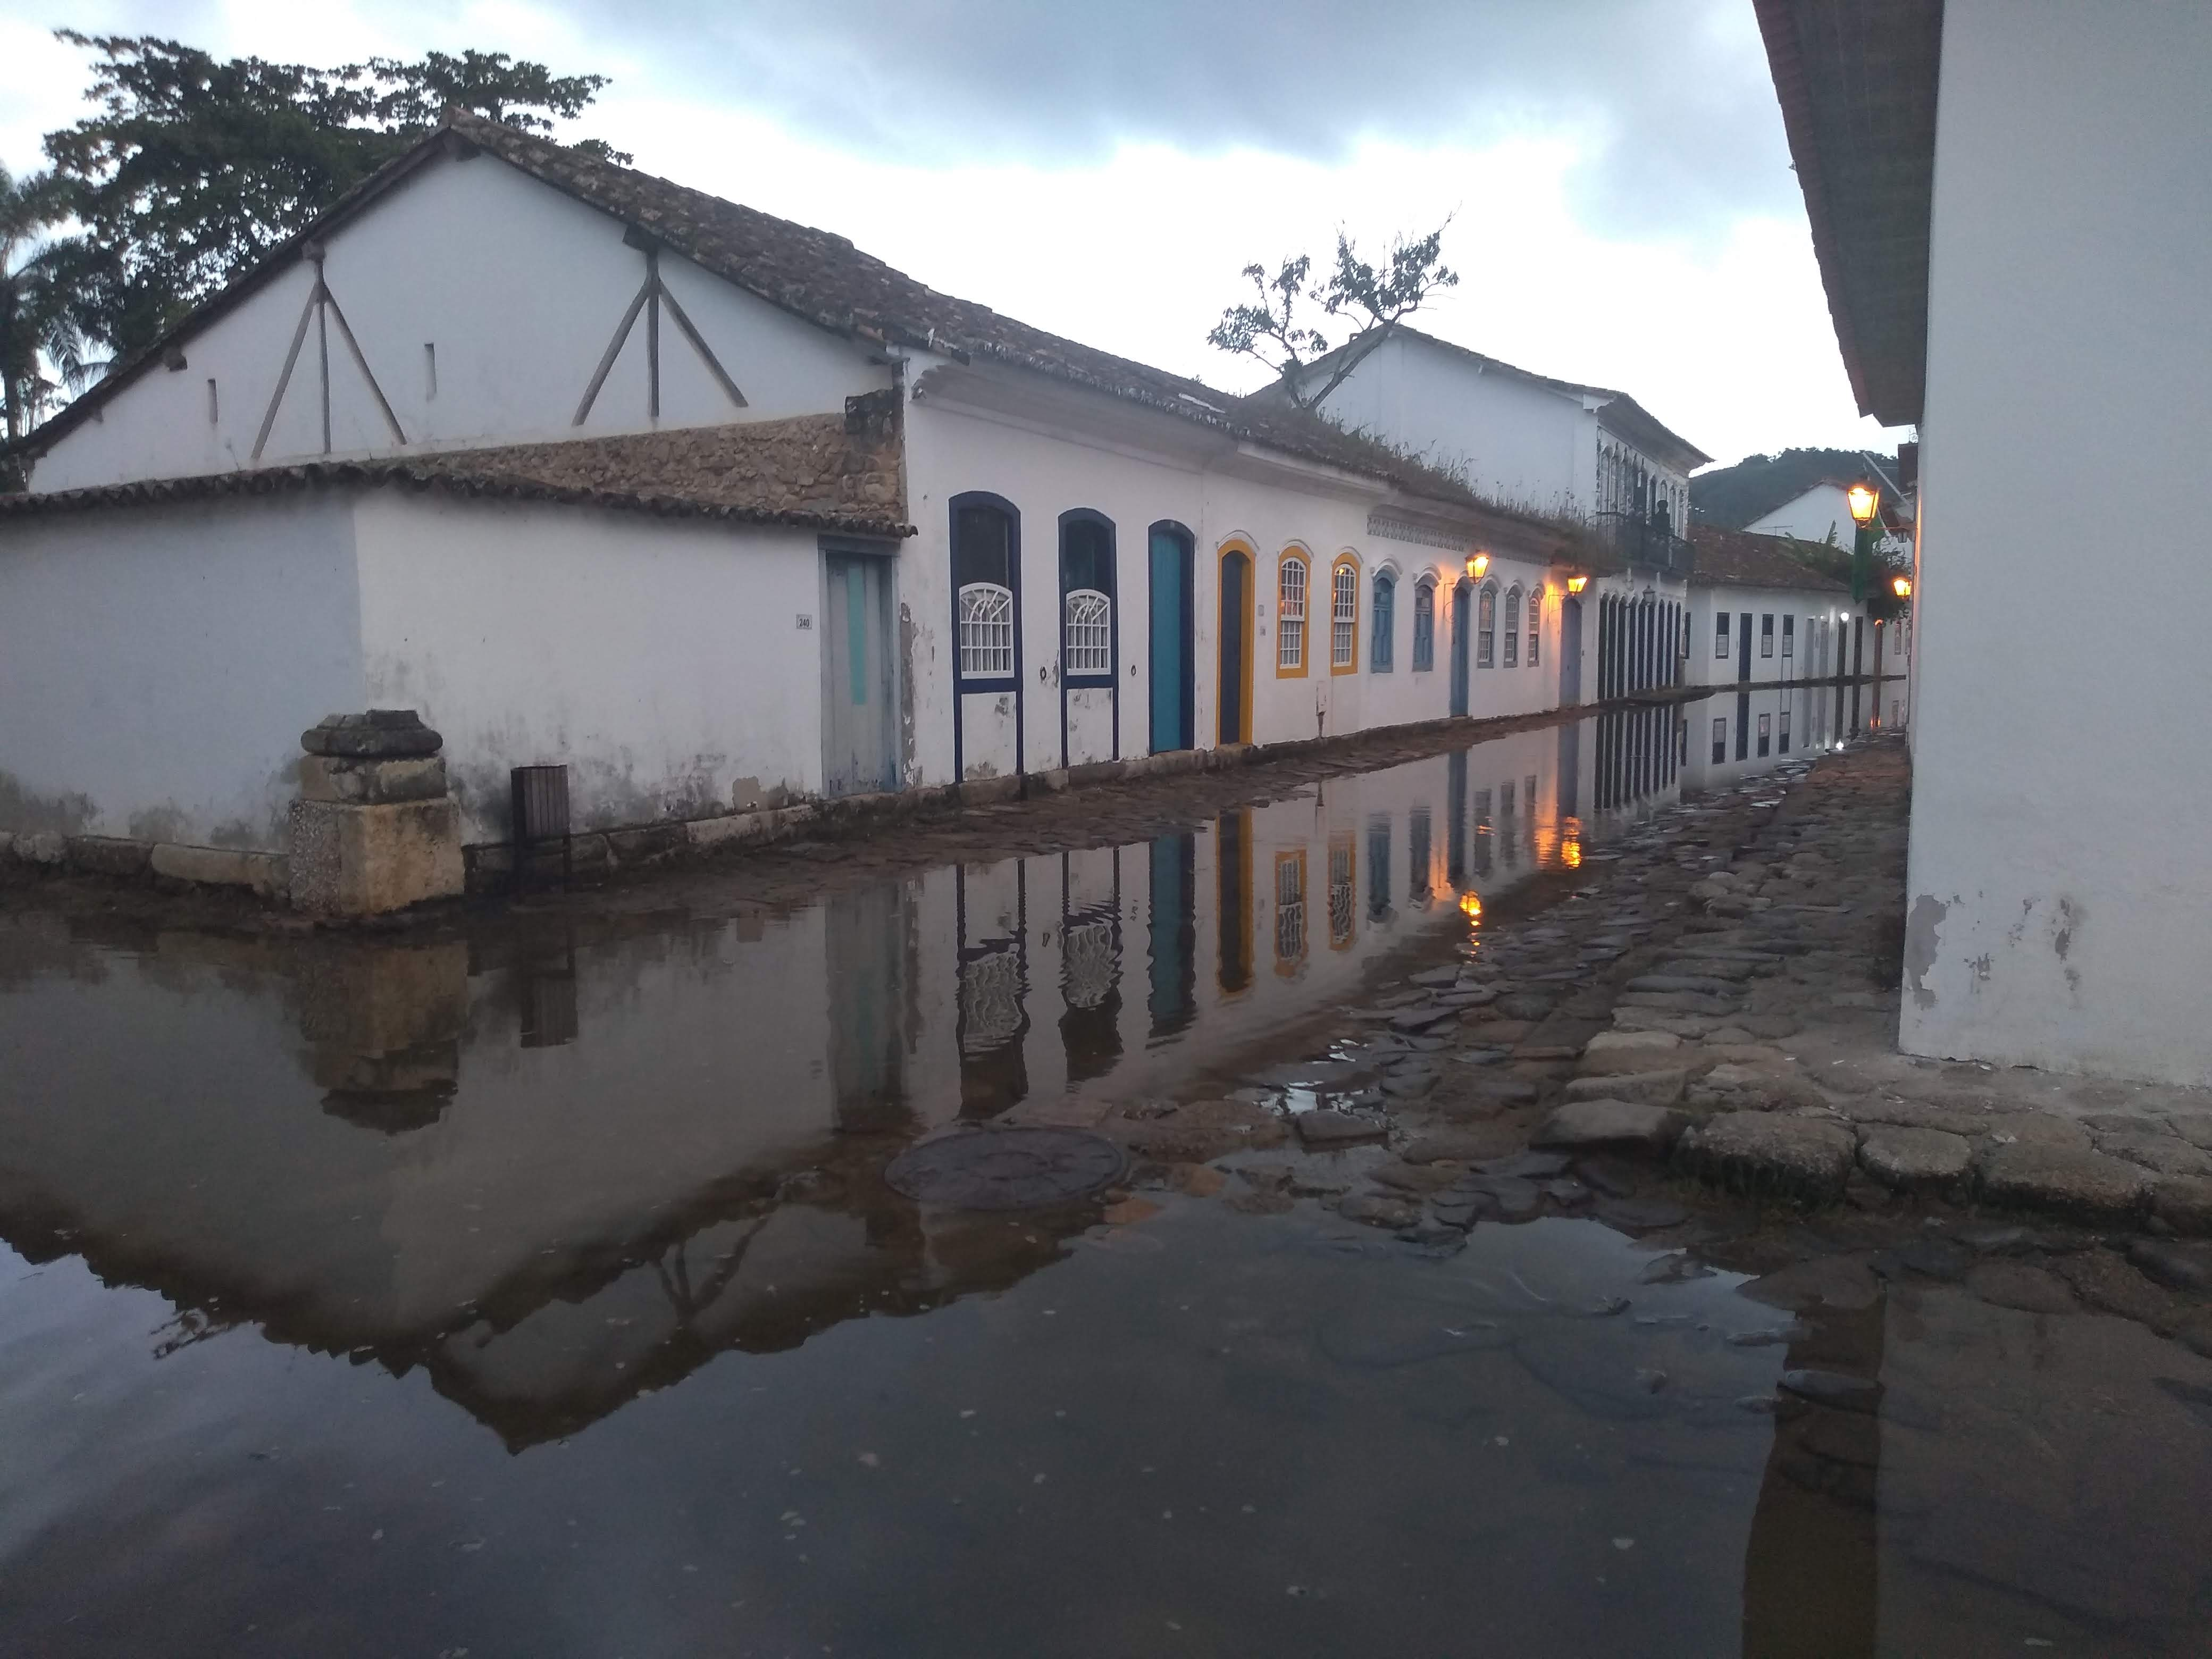
\includegraphics[height=.8\textheight]{Paraty.jpg}\caption{Paraty}
\end{figure}
}
\only<6>{
\begin{figure}
\centering
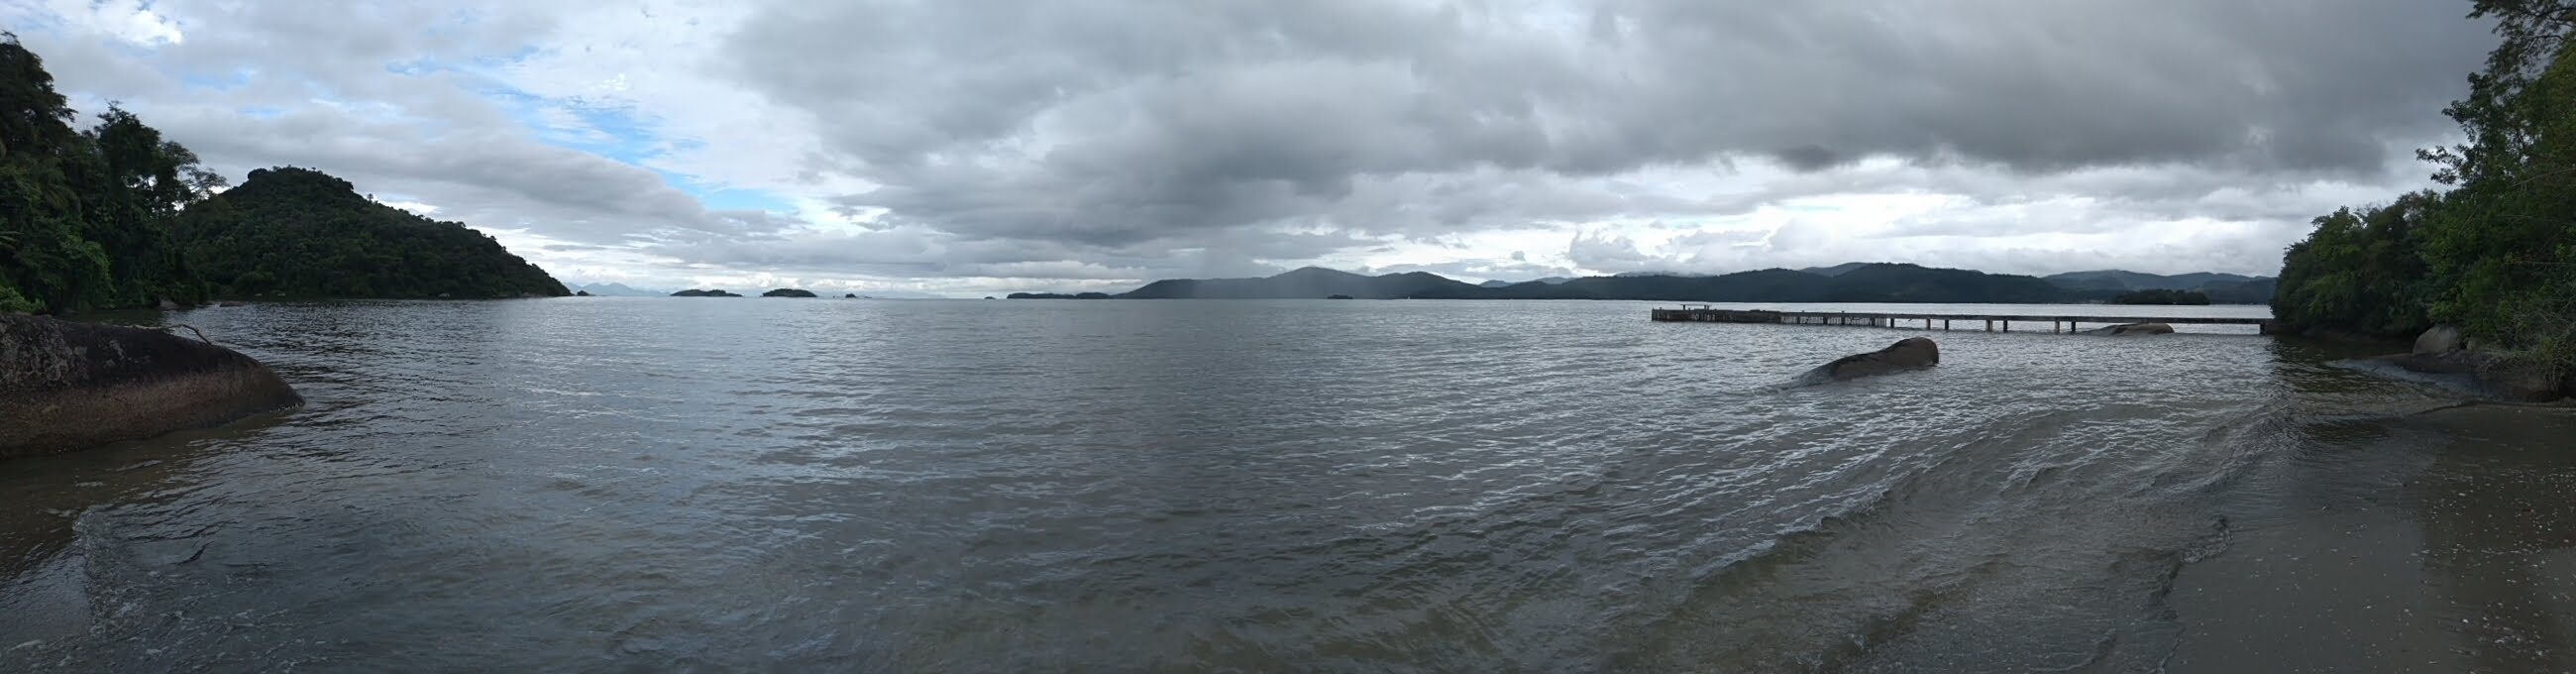
\includegraphics[width=.9\linewidth]{plage_paraty.jpg}\caption{Paraty}
\end{figure}
\begin{figure}
	\centering
	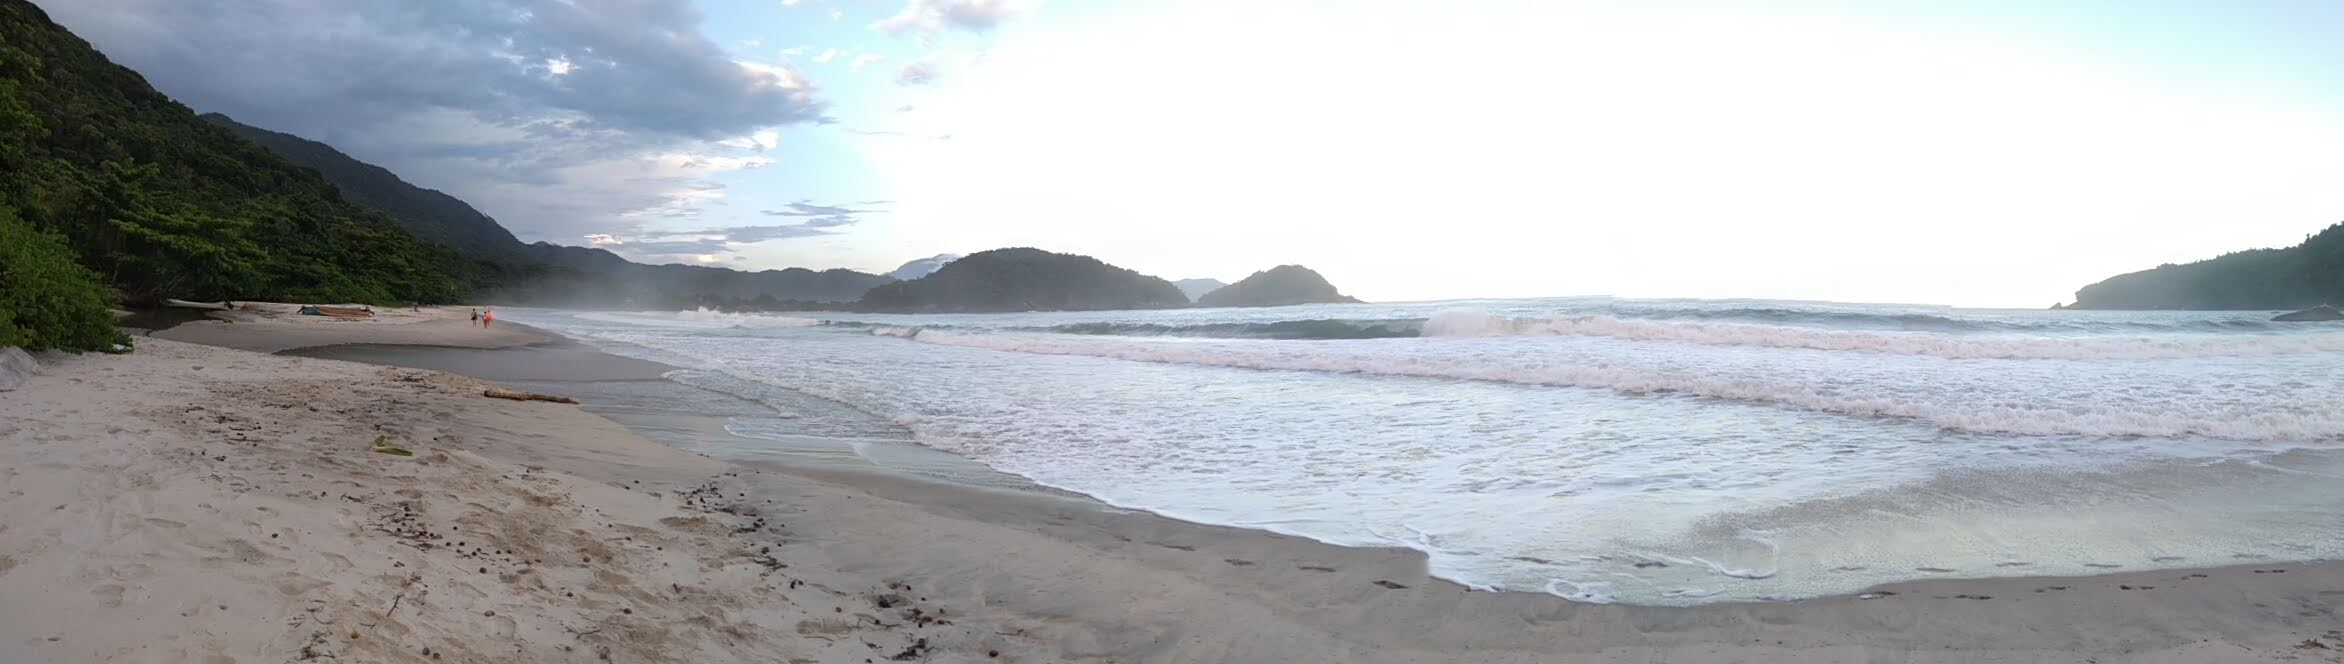
\includegraphics[width=.9\linewidth]{trinidade_plage.jpg}\caption{Trinidade}
\end{figure}
}
\only<7>{
\begin{figure}
\centering
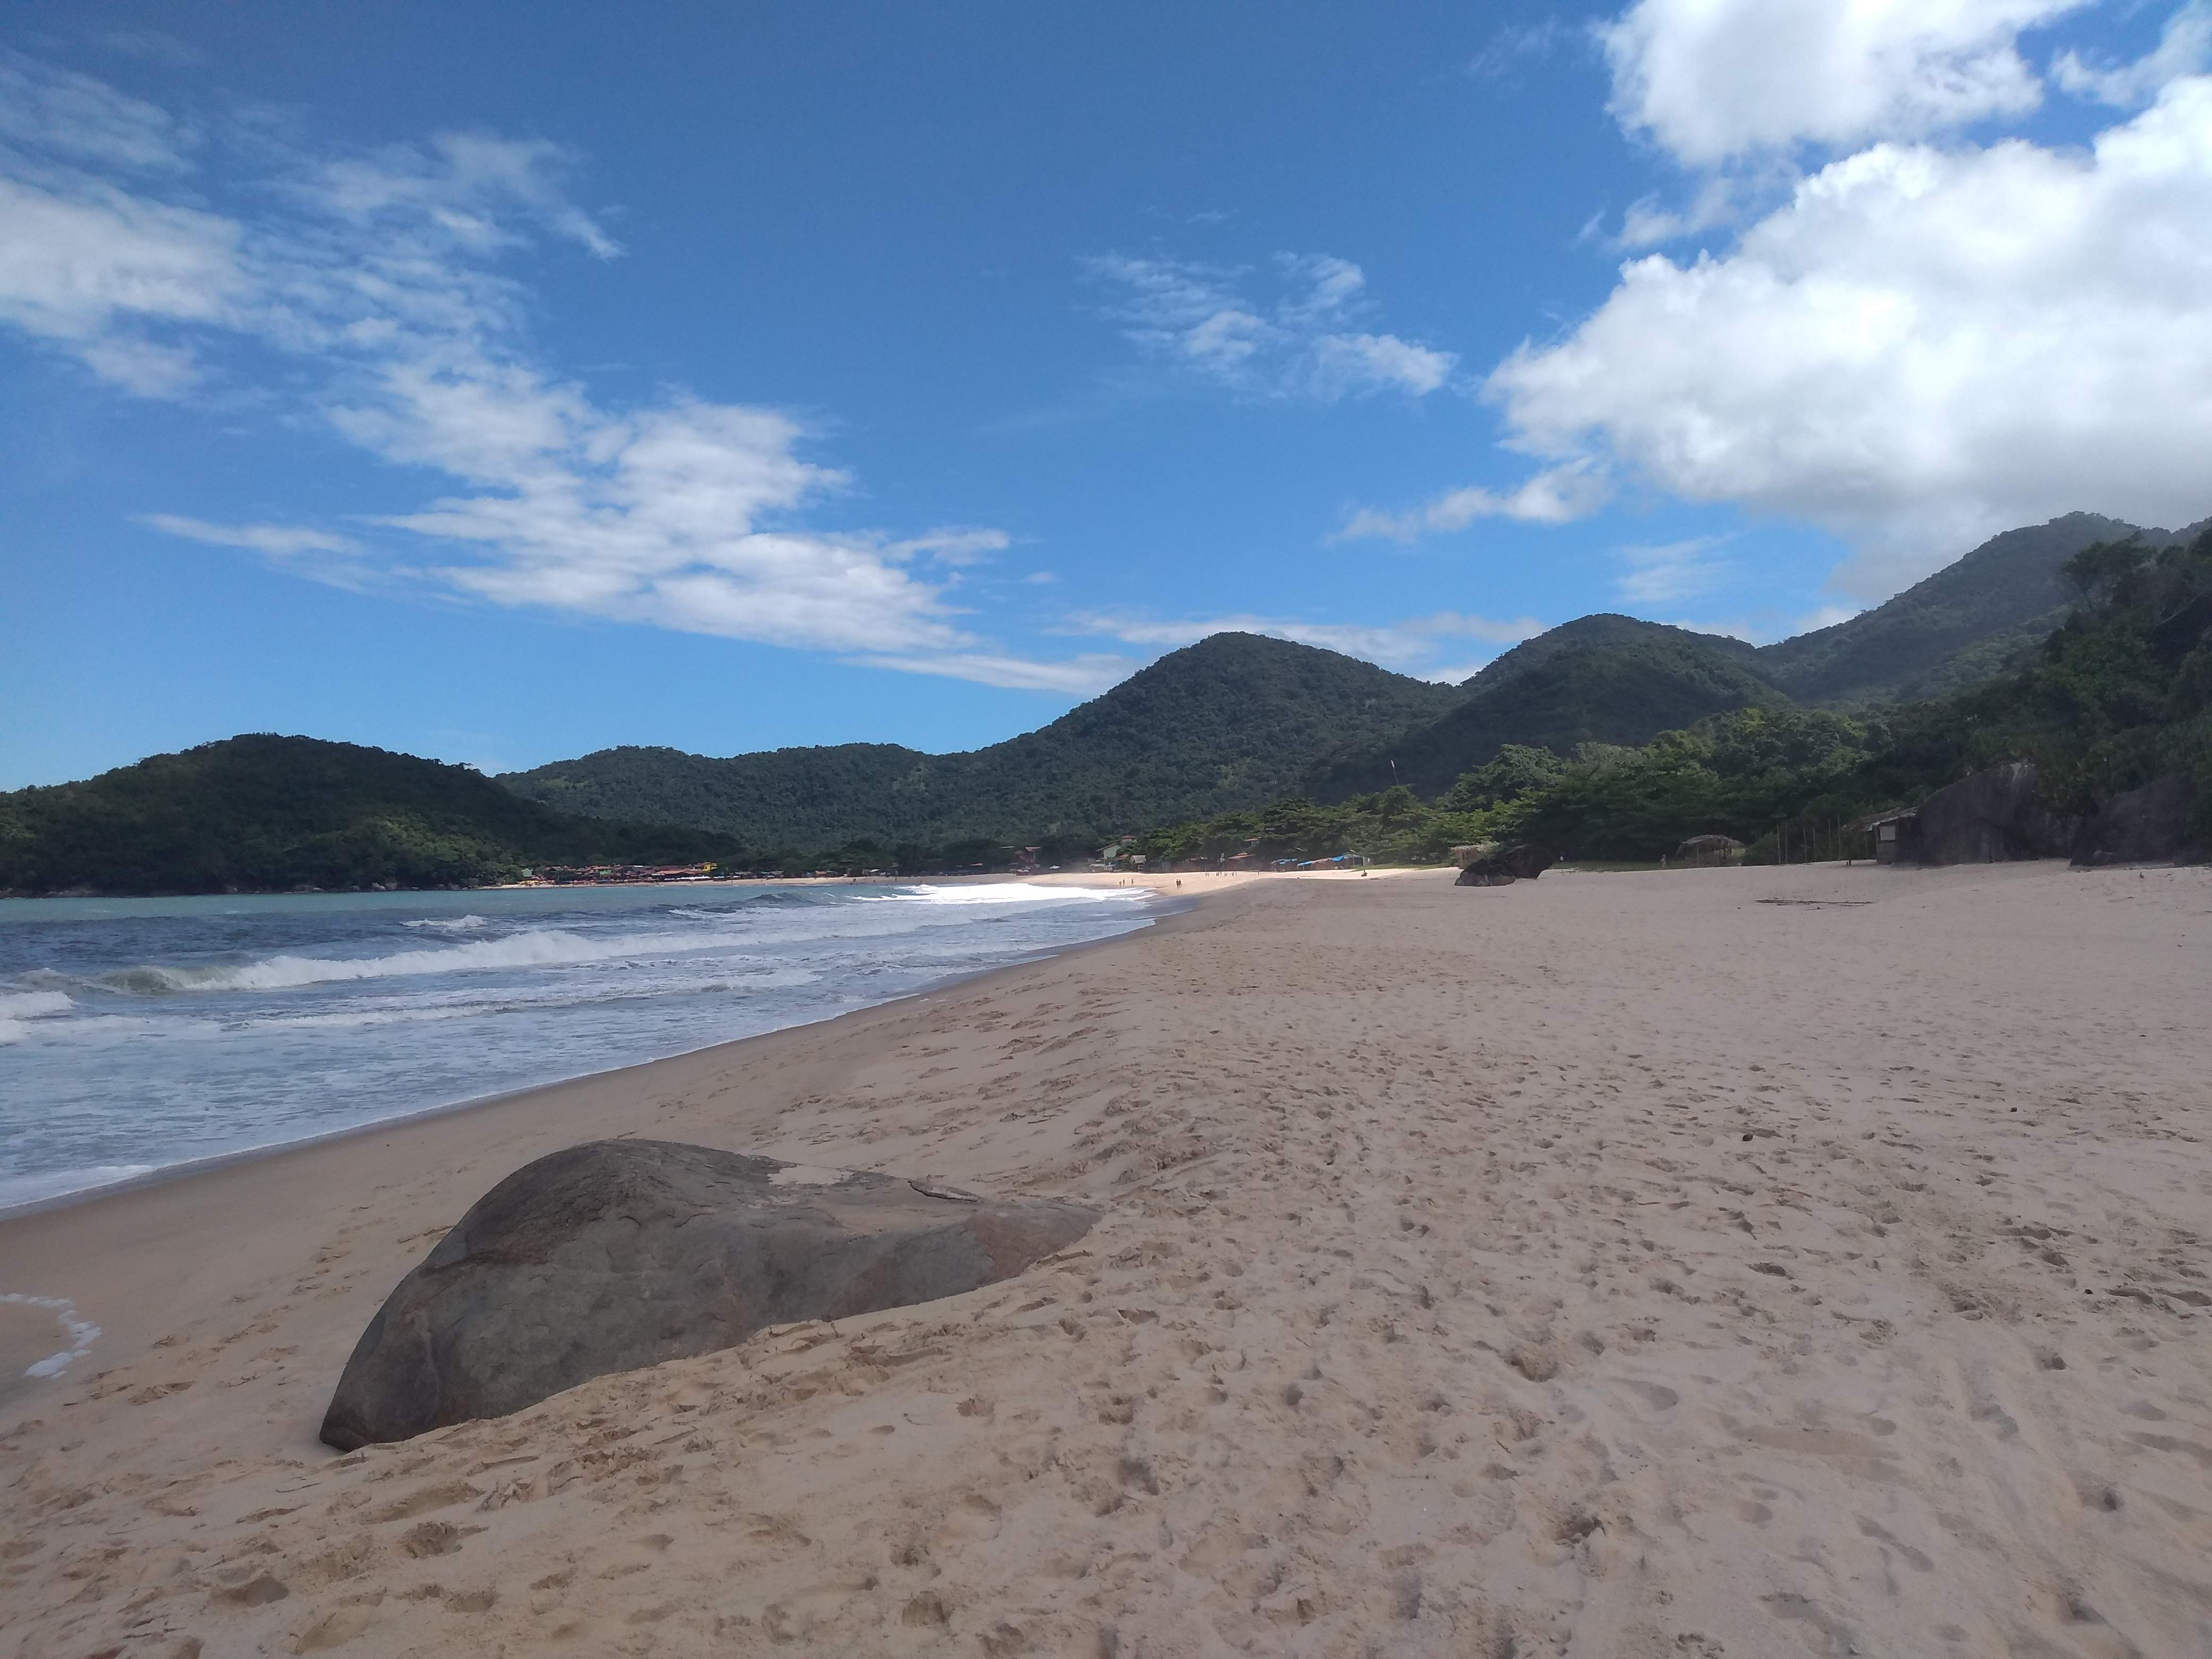
\includegraphics[height=.8\textheight]{Trinidade.jpg}\caption{Trinidade}
\end{figure}
}

\end{frame}

\section{Financer sa mobilité}
\begin{frame}{Financement EDSYS, la démarche}
Documents nécessaires:
\begin{itemize}
	\item relations antécédents avec le labo;
	\item projet de recherche;
	\item budget justifié et montant demandé à EDSYS (pour moi 4000 euro dont 1000 pour EDSYS);
	\item lettre d'invitation;
	\item présentation finale du projet (10 min);
\end{itemize}
Pensez aussi au VISA, ça peut prendre longtemps. \\
D'autres bourses peuvent démangés (bourse de la région, ISAE), renseignez vous.
\end{frame}

\begin{frame}[allowframebreaks]{Aspect recherche: publications}
\bibliographystyle{plain}
\nocite{*}
\bibliography{bib_bresil}
\end{frame}

\end{document}